\chapter{Datasets}
High dimensional datasets are not a very common research topics. In this chapter I will describe some data sources and possible applications of the described algorithm. I also show some interpretations of subspaces in different datasets and some failed approaches of finding them. To get, isolate and preprocess the data I've used some scripts. Because I think open research should not only contain open publications but also open data sources, you can find the scripts and some notes about them online.\footnote{\url{https://github.com/crepererum/GSD}} Should you have some questions, find a bug or want to contribute, feel free to use the issue tracker or file a pull request.

\section{Drug Database}
A source of high dimensional data is the list of ingredients of drugs. They collect important information about common combination of substances because one ingredient requires another, e.g. alcohol is a solvent for many chemicals. Common combinations can also be formed by combined substances that are used in drugs because manufactures produce them as a base for their product or because they act as a reseller for premixed drugs. The data set also contains information about chemicals that are never used together because they react with each other or because it does not make sense in terms of usability.

I hoped to find some public drug data bases containing drugs registered in Germany or in the EU. But this was not the case. Either they were only usable via a very limited interface or it would cost me a enormous amount of money to buy a license. Since the open data movement in USA has a very long tradition, it was easy to find an American drug database, that is easy to parse and provides a huge data collection.\footnote{\url{http://dailymed.nlm.nih.gov/dailymed/downloadLabels.cfm}} The entire data set contains \num{24094} drugs and \num{4139}. Figure~\ref{fig:drugs} visualizes a spectrum of this dataset, where rows act as drugs and image columns describe if a specific drug contains a specific substance. The most common ingredients in this data are:
\begin{itemize}
	\item water
	\item glycerin
	\item titanium dioxide
	\item propylene glycol
	\item dimethicone
\end{itemize}

\begin{figure}
	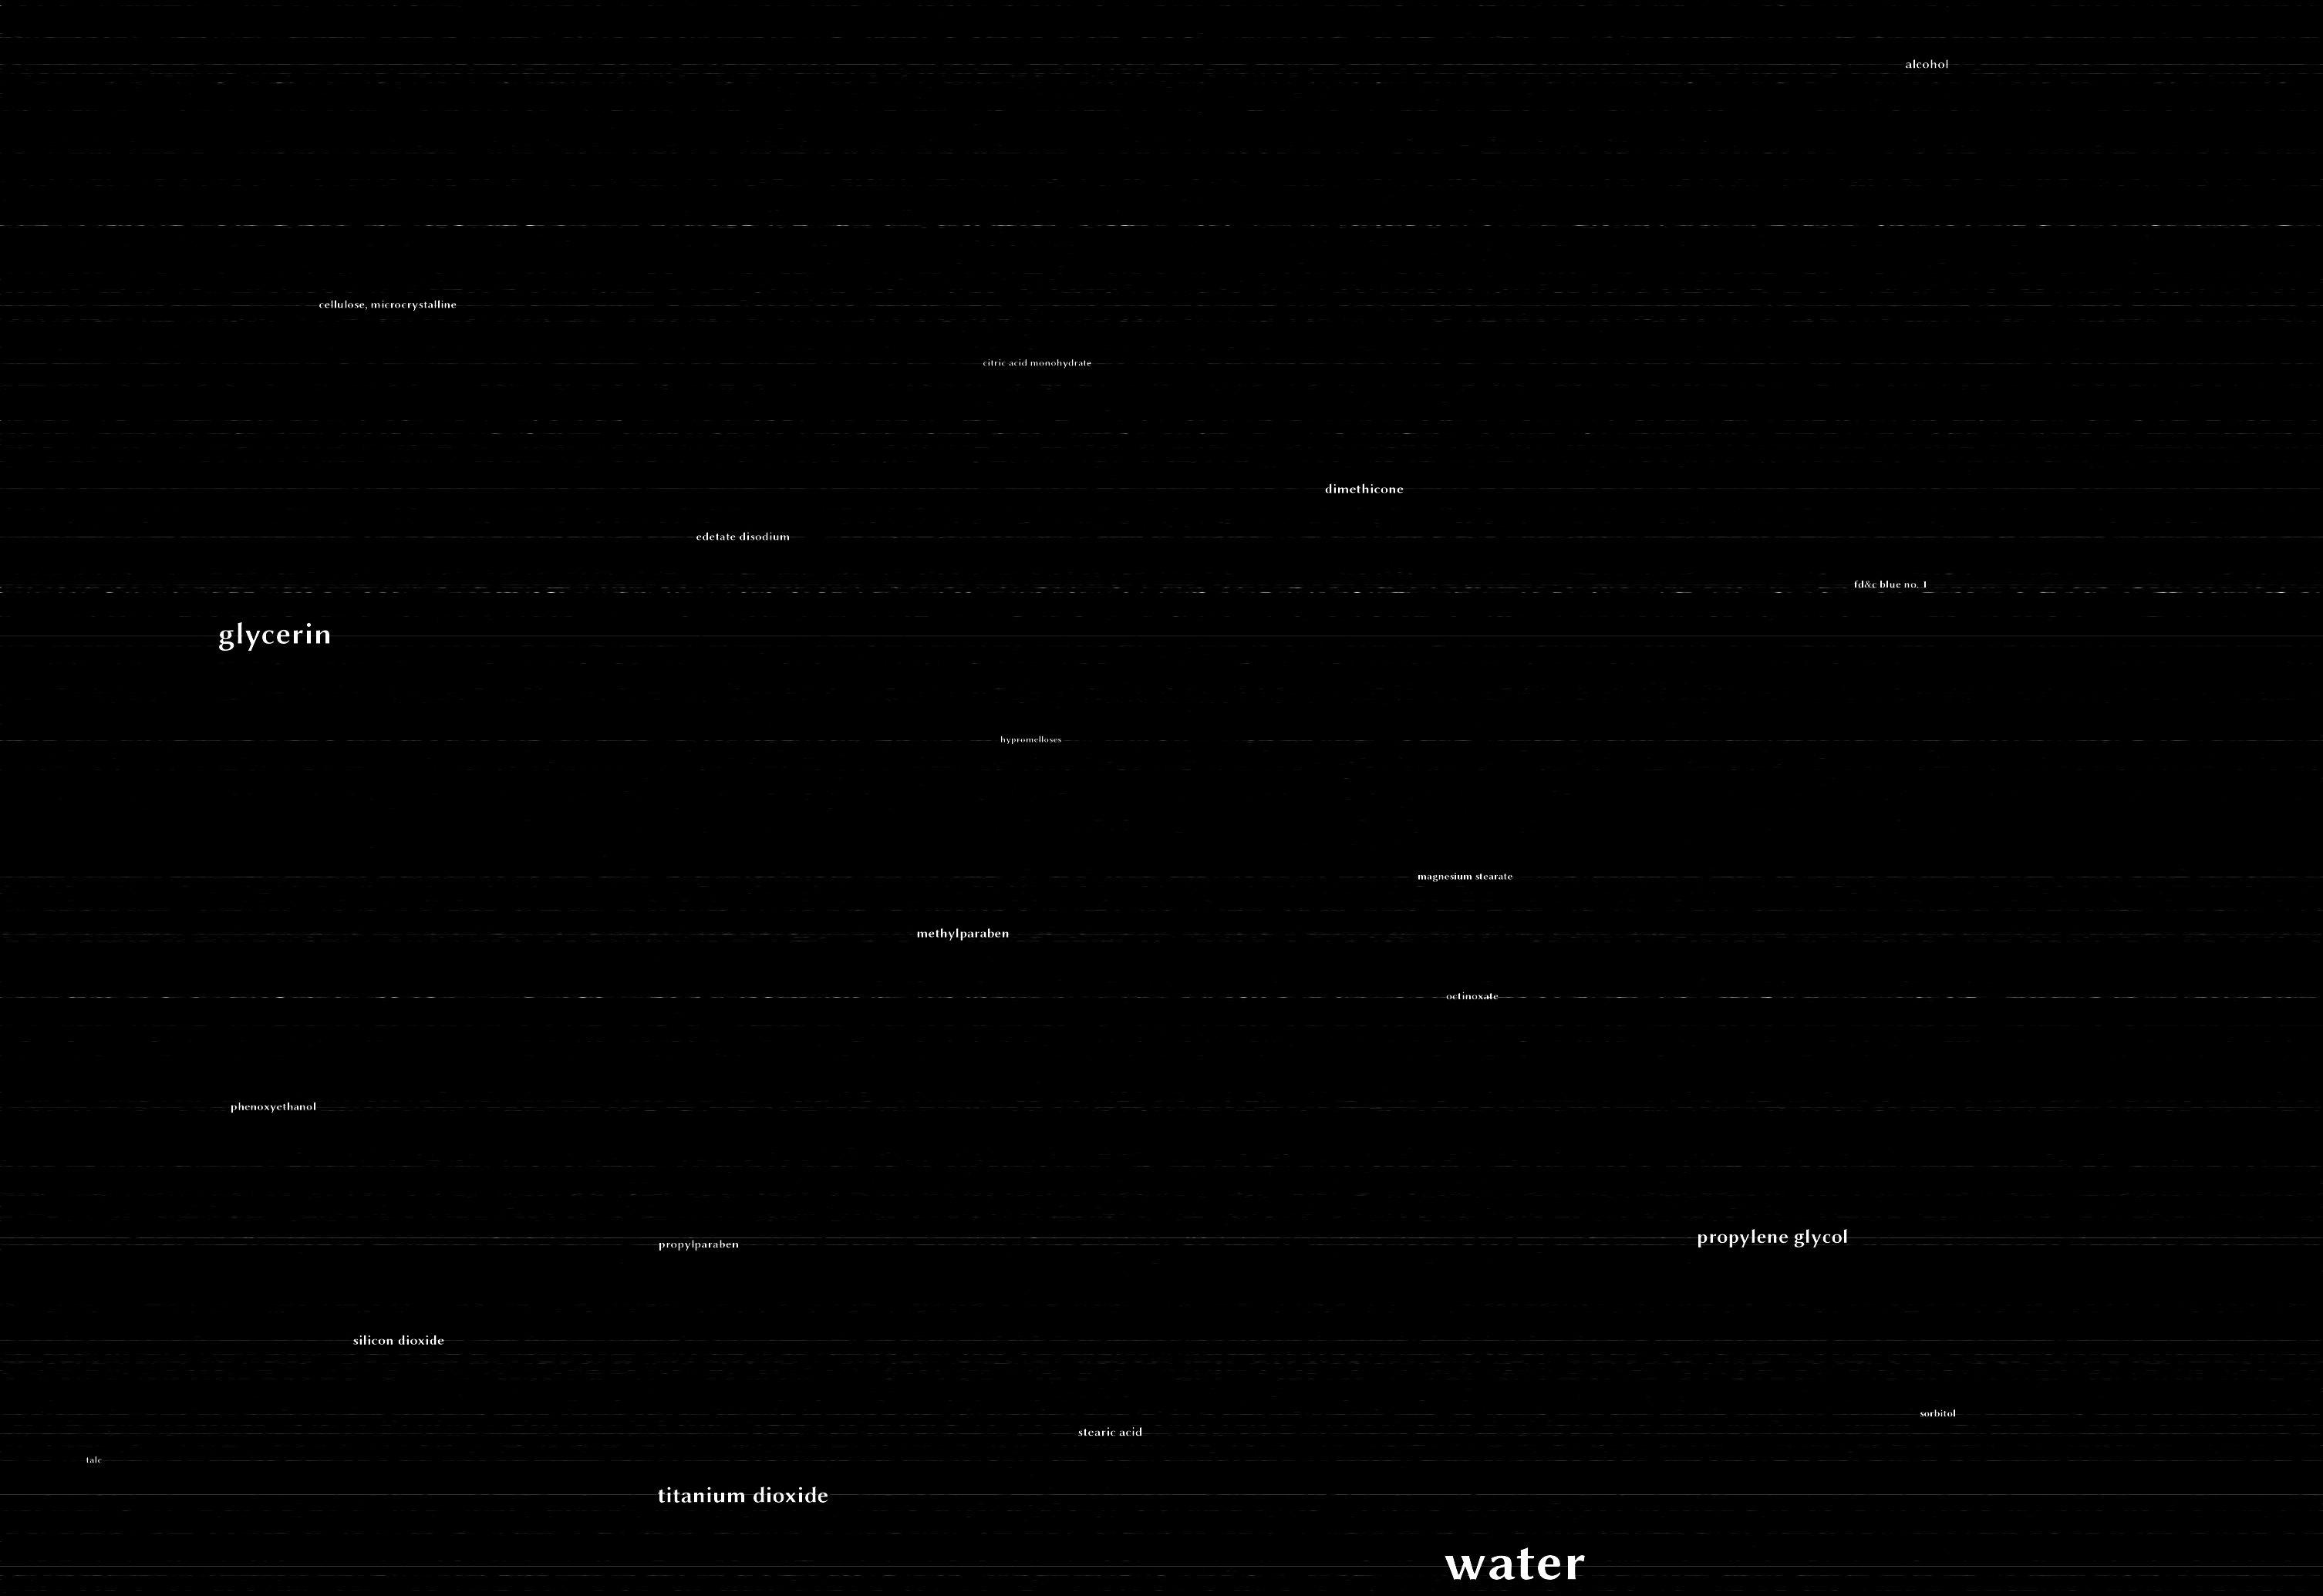
\includegraphics[height=\textheight,keepaspectratio]{drugs}
	\caption{drugs spectrum}
	\label{fig:drugs}
\end{figure}

To convert this data to a legal input data set, it is processed as followed: The only preprocessing that is done is to reduce the ingredients to their lower case text because the data set contains the same ingredients written in different combinations of lower and upper case letters. After the case normalization build a list of all ingredients in all drugs and bring them into a fixed order. Every ingredient forms one dimension. Then build a binary vector for every drug in the database where $1$ describes that a ingredient is contained in the drug and $0$ if this is not the case. I provide a parser and converter for this kind of data.

GraBaSS is used with $t_e = 0.25$, $t_n = 0.65$ and $d = 3$. It extracts many subspaces, that describe rare combinations, that are used in some natural products. The listed substances are also natural, e.g. leafs, flowers and roots. Because the ingredients are so uncommon, they form subspaces when only used together only a few times. Trying to eliminate this substances is not possible without loosing most of the data set because there are only a few substances that are very common and many that are uncommon.

Some examples for more usable subspaces are:
\begin{itemize}
	\item boron, bromine, lithium, magnesium, manganese, potassium, sodium, strontium
	\item alanine, asparagine, cysteine, histidine, ornithine, threonine
\end{itemize}

ENCLUS extracted very small subspaces. When increasing $\epsilon$, the algorithm does not finish within hours because the data set is too large. So I got no usable results.

